\subsection{Taxonomy-topic model}\label{sec:taxonomy_analysis}\todo{snak om appendix stuff til sidst i dette afsnit(linje 3 skal rykkes), og lav tabel med de topics vi snakker om}
Finally, we also want to analyze the taxonomy-topic model, especially since this model has the highest topic coherence out of all the tested models.
\autoref{tab:pachinko_topics} in the appendix shows the final lowest level topics of the taxonomy-topic model.
Note that, while most of the topics are semantically coherent, there are some topics (e.g., topic 19 and 42) that consist entirely of words that provide little context or semantic meaning.
This indicates that the model has learned to group words that do not belong to any good topics.
This is a good feature that allows the model to apply an extra layer of preprocessing, automatically filtering away irrelevant words into topics.
This feature is also seen in some other topic models, such as in the hierarchical \gls{lda} (hLDA) by \citet{hLDA2004} and the embedded topic model (ETM) by \citet{dieng2020topic}, but the \gls{lda} does not seem to have this feature.

Since this model deals with more topic distributions than the other models, it is worth checking whether it also converges within the first 50 epochs, as with \gls{lda}.
This does seem to be the case, as indicated by \autoref{fig:pachinko_train}.
Here it can be seen that the topic coherence curve has flattened significantly, and thus additional epochs will have diminishing returns.\vejleder{what about LL?}

\begin{figure}
	\centering
	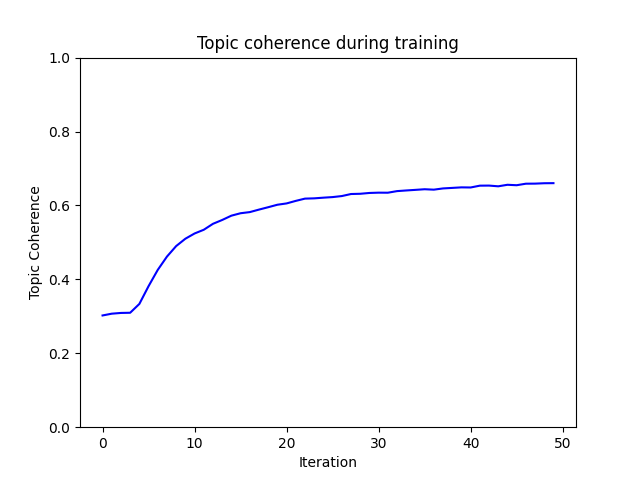
\includegraphics[width= \linewidth]{figures/pachinko_training.PNG}
	\caption{Topic coherence during training of the taxonomy-topic model.}
	\label{fig:pachinko_train}
\end{figure}

\autoref{tab:pachinko_mid_topics} gives an overview of how the taxonomy topics in the third layer of the taxonomy-topic model, are connected to the fourth layer topics that were generated by the model.
Some of these connections make a lot of sense, such as the 'Økonomi' (Economy) topic which has the three filler\vejleder{explain filler} topics: 79, 75, and 42, which consists of words with little semantic value, and two topics which are about money: 74 and 9.
However not all the connections\vejleder{the connections make er understreget} make as much sense as these. 
For example, the 'Kriminalitet' (Crime) topic has two filler topics: 42 and 75, one topic about economy: 60, one topic about politics: 8, and one topic about sports: 86.
See \autoref{tab:pachinko_topics}, for more details on the top words within each of these topics.
\vejleder{uddyb gerne}
Having the layered structure of the \gls{pam} gives many possibilities for recommending new articles to readers.
There is the possibility of exploring the similarity of taxonomies at the same layer and using this to recommend new articles with similar subjects.
For example, if an article is about 'Miljø' (environment) similar taxonomies might be 'Natur' (nature) and possibly 'Etik' (ethics), 'Trafik' (traffic), and 'Energi' (energy).

\begin{table*}[h]
	\centering
	\caption{IDs of the top 5 most occurring fourth layer topics for each third layer topic from the pachinko model. See \autoref{tab:pachinko_topics} for the most occurring words for each ID.}
	\label{tab:pachinko_mid_topics}
	\begin{tabular}{c | c | c | c | c | c}
		Taxonomy Name & Top 5 Topic IDs & Taxonomy Name & Top 5 Topic IDs & Taxonomy Name & Top 5 Topic IDs \\ \hline
		Danmark & 8, 42, 82, 59, 79 & Udland & 42, 79, 59, 8, 32 & Kultur & 9, 42, 79, 19, 8 \\
		Landbrug & 42, 79, 8, 9, 19 & Kriminalitet & 42, 75, 60, 8, 86 & Socialstof & 42, 9, 79, 86, 8 \\
		Arbejdsmarked & 42, 79, 59, 8, 9 & Økonomi & 79, 75, 74, 42, 9 & Sundhed & 8, 32, 42, 9, 19 \\
		Politik & 42, 75, 9, 19, 74 & Musik & 75, 42, 59, 11, 79 & Sport & 42, 75, 8, 59, 52 \\
		Bolig & 75, 42, 86, 79, 8 & Videnskab & 42, 8, 52, 79, 19 & Trafik & 42, 74, 8, 52, 32 \\
		Erhverv & 42, 8, 59, 32, 79 & Uddannelse & 42, 9, 75, 32, 74 & Energi & 42, 8, 79, 19, 86 \\
		Ulykker & 42, 75, 9, 79, 32 & Fritid & 42, 8, 75, 82, 79 & Socialt & 42, 75, 79, 59, 9 \\
		Dyr & 86, 42, 79, 52, 9 & Natur & 42, 52, 9, 32, 79 & Miljø & 8, 42, 75, 52, 59 \\
		Familie & 79, 8, 42, 59, 32 & Politi & 42, 75, 79, 8, 59 & Byggeri & 75, 42, 79, 77, 59 \\
		Etik & 79, 42, 8, 86, 74 & Religion & 42, 79, 8, 59, 32 & Kommunalvalg & 42, 8, 75, 79, 32 \\
		Nordjyske Plus & 42, 86, 9, 79, 74 & DF & 42, 8, 59, 52, 19 & & \\
	\end{tabular}
\end{table*}
